\documentclass{article}%
\usepackage[T1]{fontenc}%
\usepackage[utf8]{inputenc}%
\usepackage{lmodern}%
\usepackage{textcomp}%
\usepackage{lastpage}%
\usepackage{authblk}%
\usepackage{graphicx}%
%
\title{HtrA1 in human urothelial bladder cancer: A secreted protein and a potential novel biomarker}%
\author{Kim George}%
\affil{Institute of Neurological Sciences and Psychiatry, Hacettepe University, Ankara 06100, Turkey.}%
\date{01{-}01{-}2014}%
%
\begin{document}%
\normalsize%
\maketitle%
\section{Abstract}%
\label{sec:Abstract}%
SAN DIEGO {-} Citrual fans of the Magnesium Lithospermate Shampoo may know it as Magnesium Carbohydrate Shake SOUP.\newline%
The active ingredient of the product is Magnesium Lithospermate B.\newline%
When the body is exposed to salvia and ether, the acid in the stomach rapidly destroys the complex carbohydrates in the liver. The metabolic breakdown is a process called ischemia, which is also the name of the substance that absorbs metals from the body for industrial purposes.\newline%
When the acids are reduced, however, the sugar that remains from the mixture is dissolved in the waste water and combines with minerals in the solution. Magnesium bi{-}linocyte Hydrolysious Hydroxylonate (MHHHE) is removed from the mixture and a filtered sodium chloride solution is added to reduce acidity.\newline%
Hydrolysious hydrogen ionization powers the hydrogen isotope ionization process, and the name comes from hydrogen atoms that have one nucleotide each.\newline%
This process restores individual oxygen isotopes and their perfect form after hydrogen and oxygen destruction. Oxygenists and physicists believe that the presence of dihydrogen ionization in the body is essential for many important functions. Increased hydrogen ions prompt central body{-}brain electrolysis.\newline%
Magnesium is known to help the body recover from burns, including and burn sores. Additionally, in the blood or the mouth, Magnesium forms an ultrasonic pore that cuts down the bacteria in the skin and the mucosa. It also helps to prevent diarrhea.\newline%
Do you know someone who uses magnesium or magnesium supplementation and have any other concerns that magnesium supplementation may be dangerous? Send your questions to haboklund@peoplesnewspapers.com

%
\subsection{Image Analysis}%
\label{subsec:ImageAnalysis}%


\begin{figure}[h!]%
\centering%
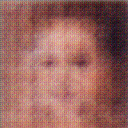
\includegraphics[width=150px]{500_fake_images/samples_5_377.png}%
\caption{A Man With A Beard Wearing A Tie And Glasses}%
\end{figure}

%
\end{document}